%======================================================================
\subsection{BW-SIM-07 P1 --- Built, 1 Nov: the Model Builder and the Settings pane}\label{sec:sim07-gui-built}
%======================================================================

The two panes of the Simulation workspace are filled (all Python: \file{bruceworx\_sim\_panes.py}, on top of the headless
\file{bruceworx\_sim\_model.py} and the shell \file{bruceworx\_sim\_workspace.py}). The layout is the one you chose on
1 Nov, not the three columns of the plan: one left sidebar with tabs, the Model Builder on top of Settings.

\begin{figure}[!htbp]
\centering
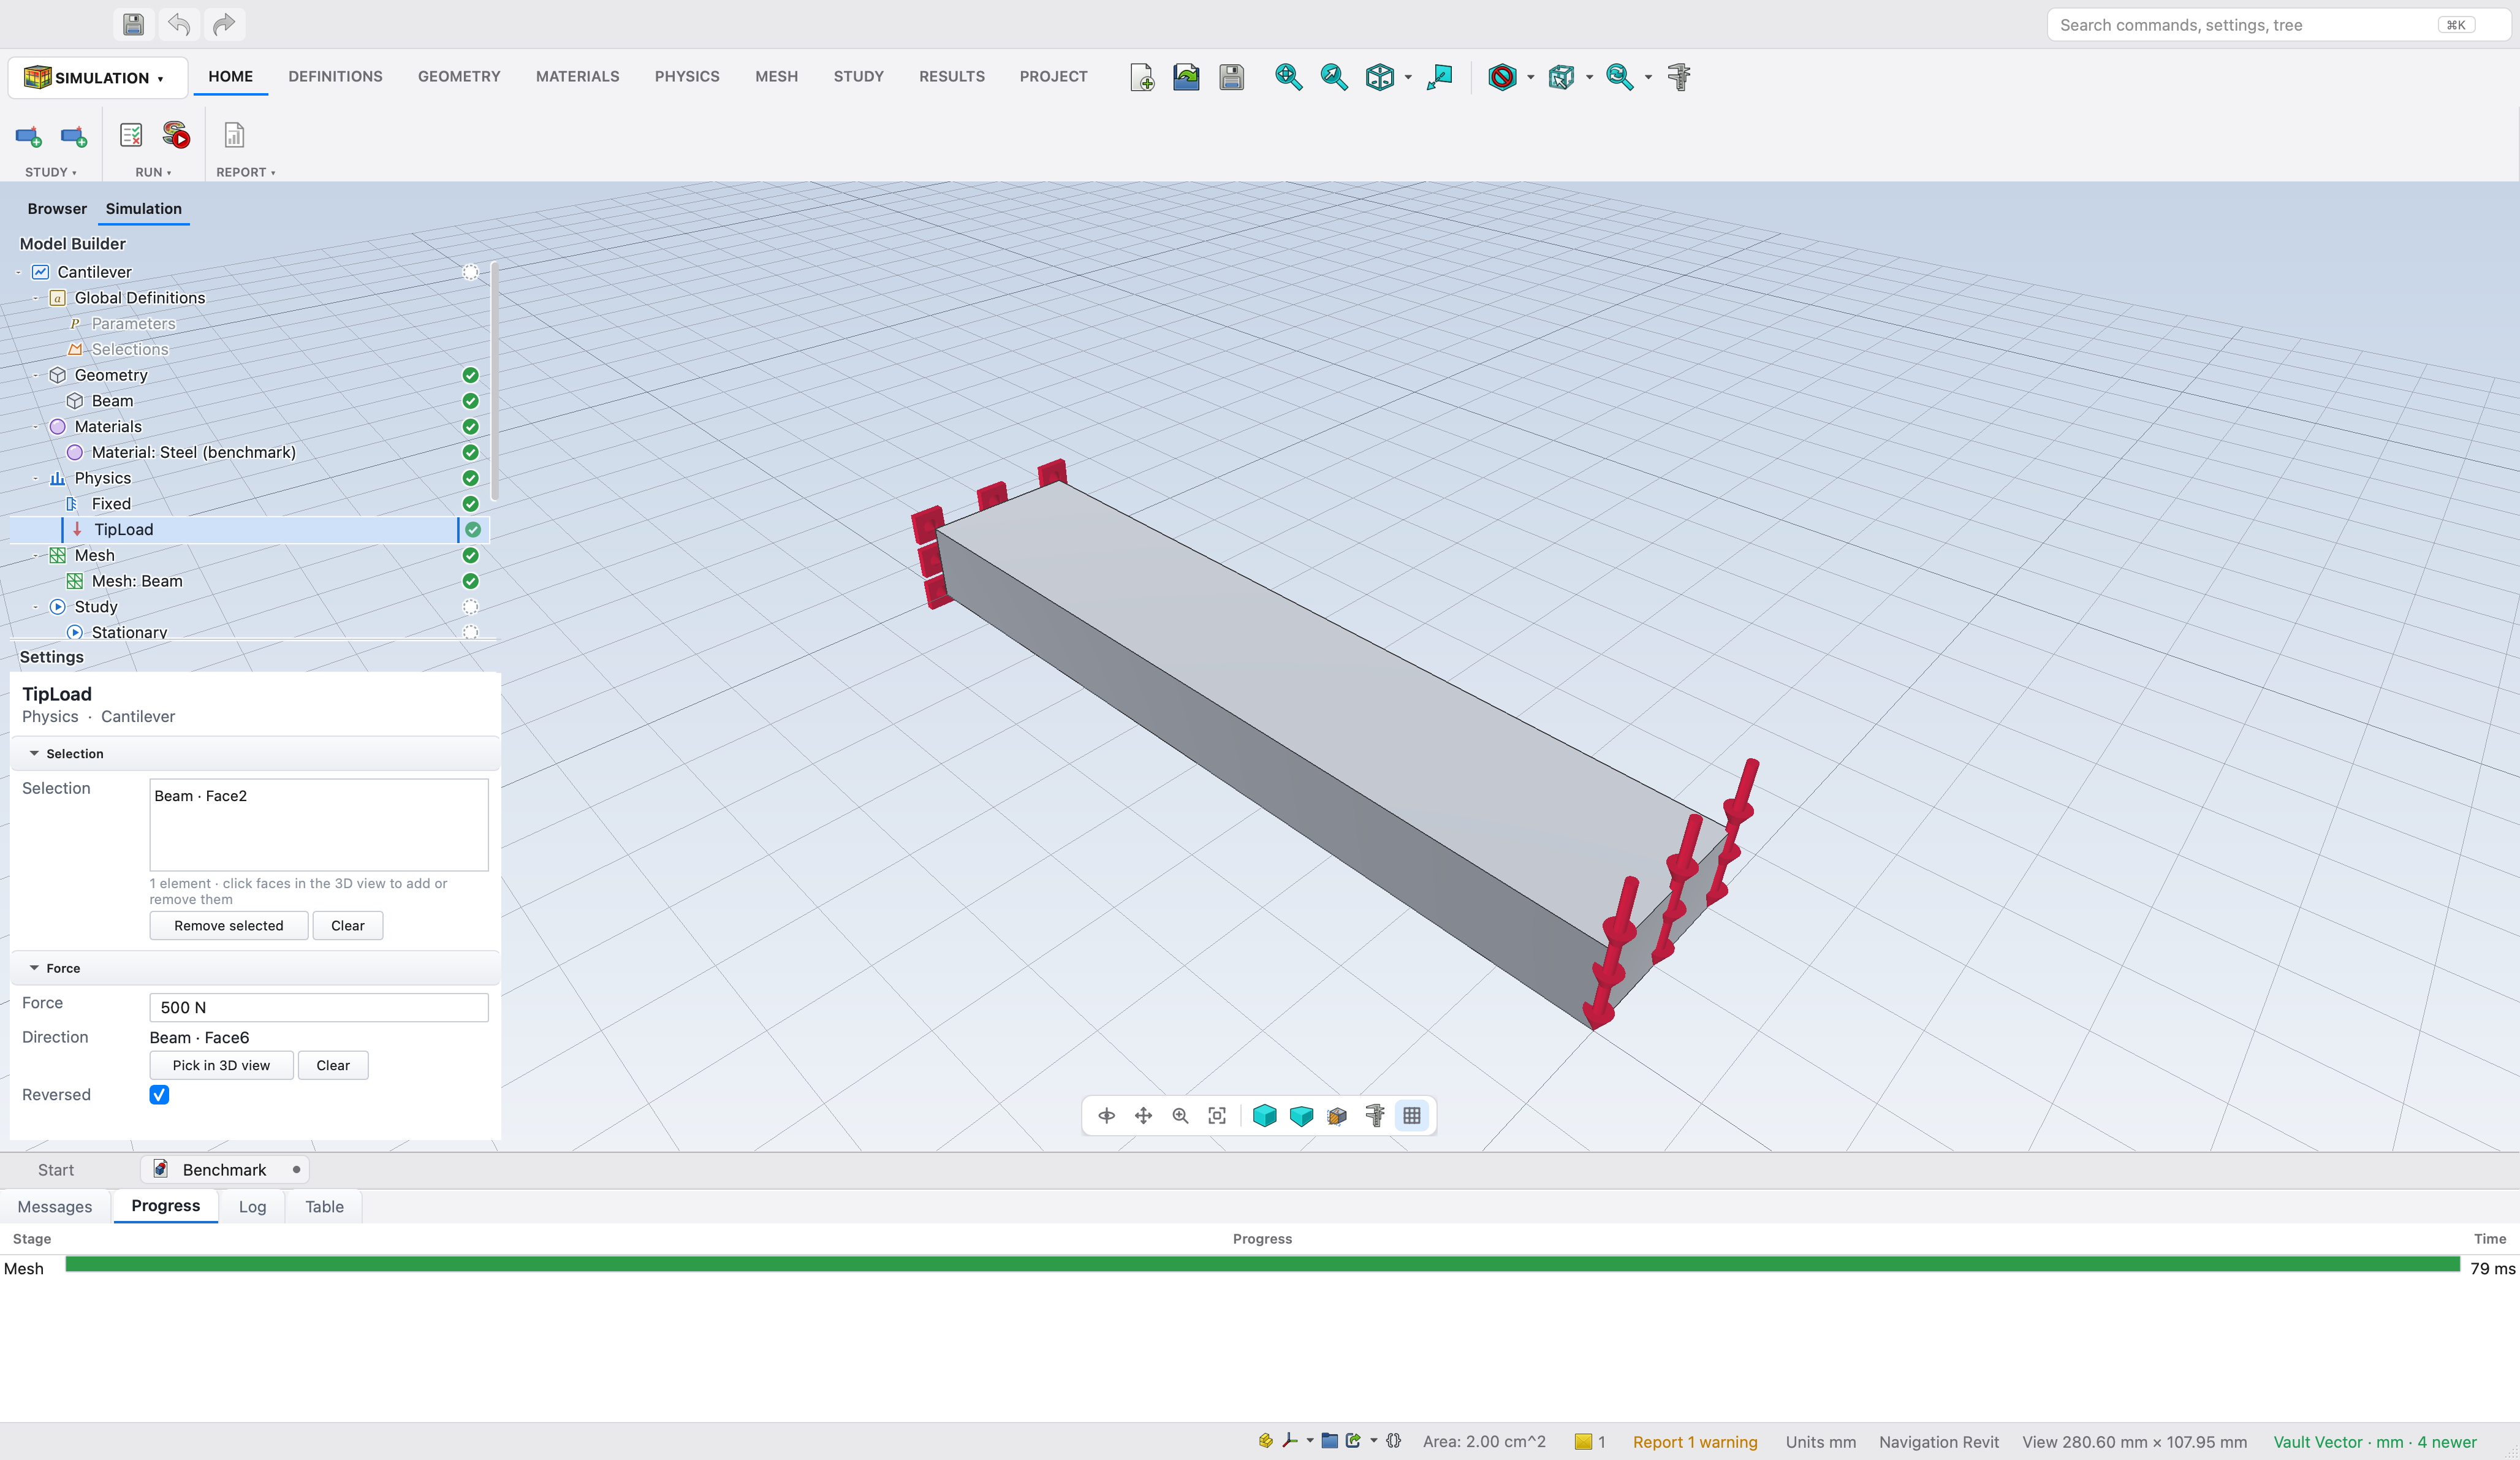
\includegraphics[width=\linewidth]{fig/simui_p1_setup.png}
\caption{Setting up the cantilever (off-screen render of the real window): the left sidebar has a horizontal tab strip, Browser (the
model tree) | Simulation; in the Simulation tab the Model Builder (state marks at the right of each row) is over the
Settings of the selected node (\emph{TipLoad}: its faces, the force, its direction). The step ribbon shows no Study or
Results tab group beyond Run and Report.}
\label{fig:sim07-gui-setup}
\end{figure}

\begin{figure}[!htbp]
\centering
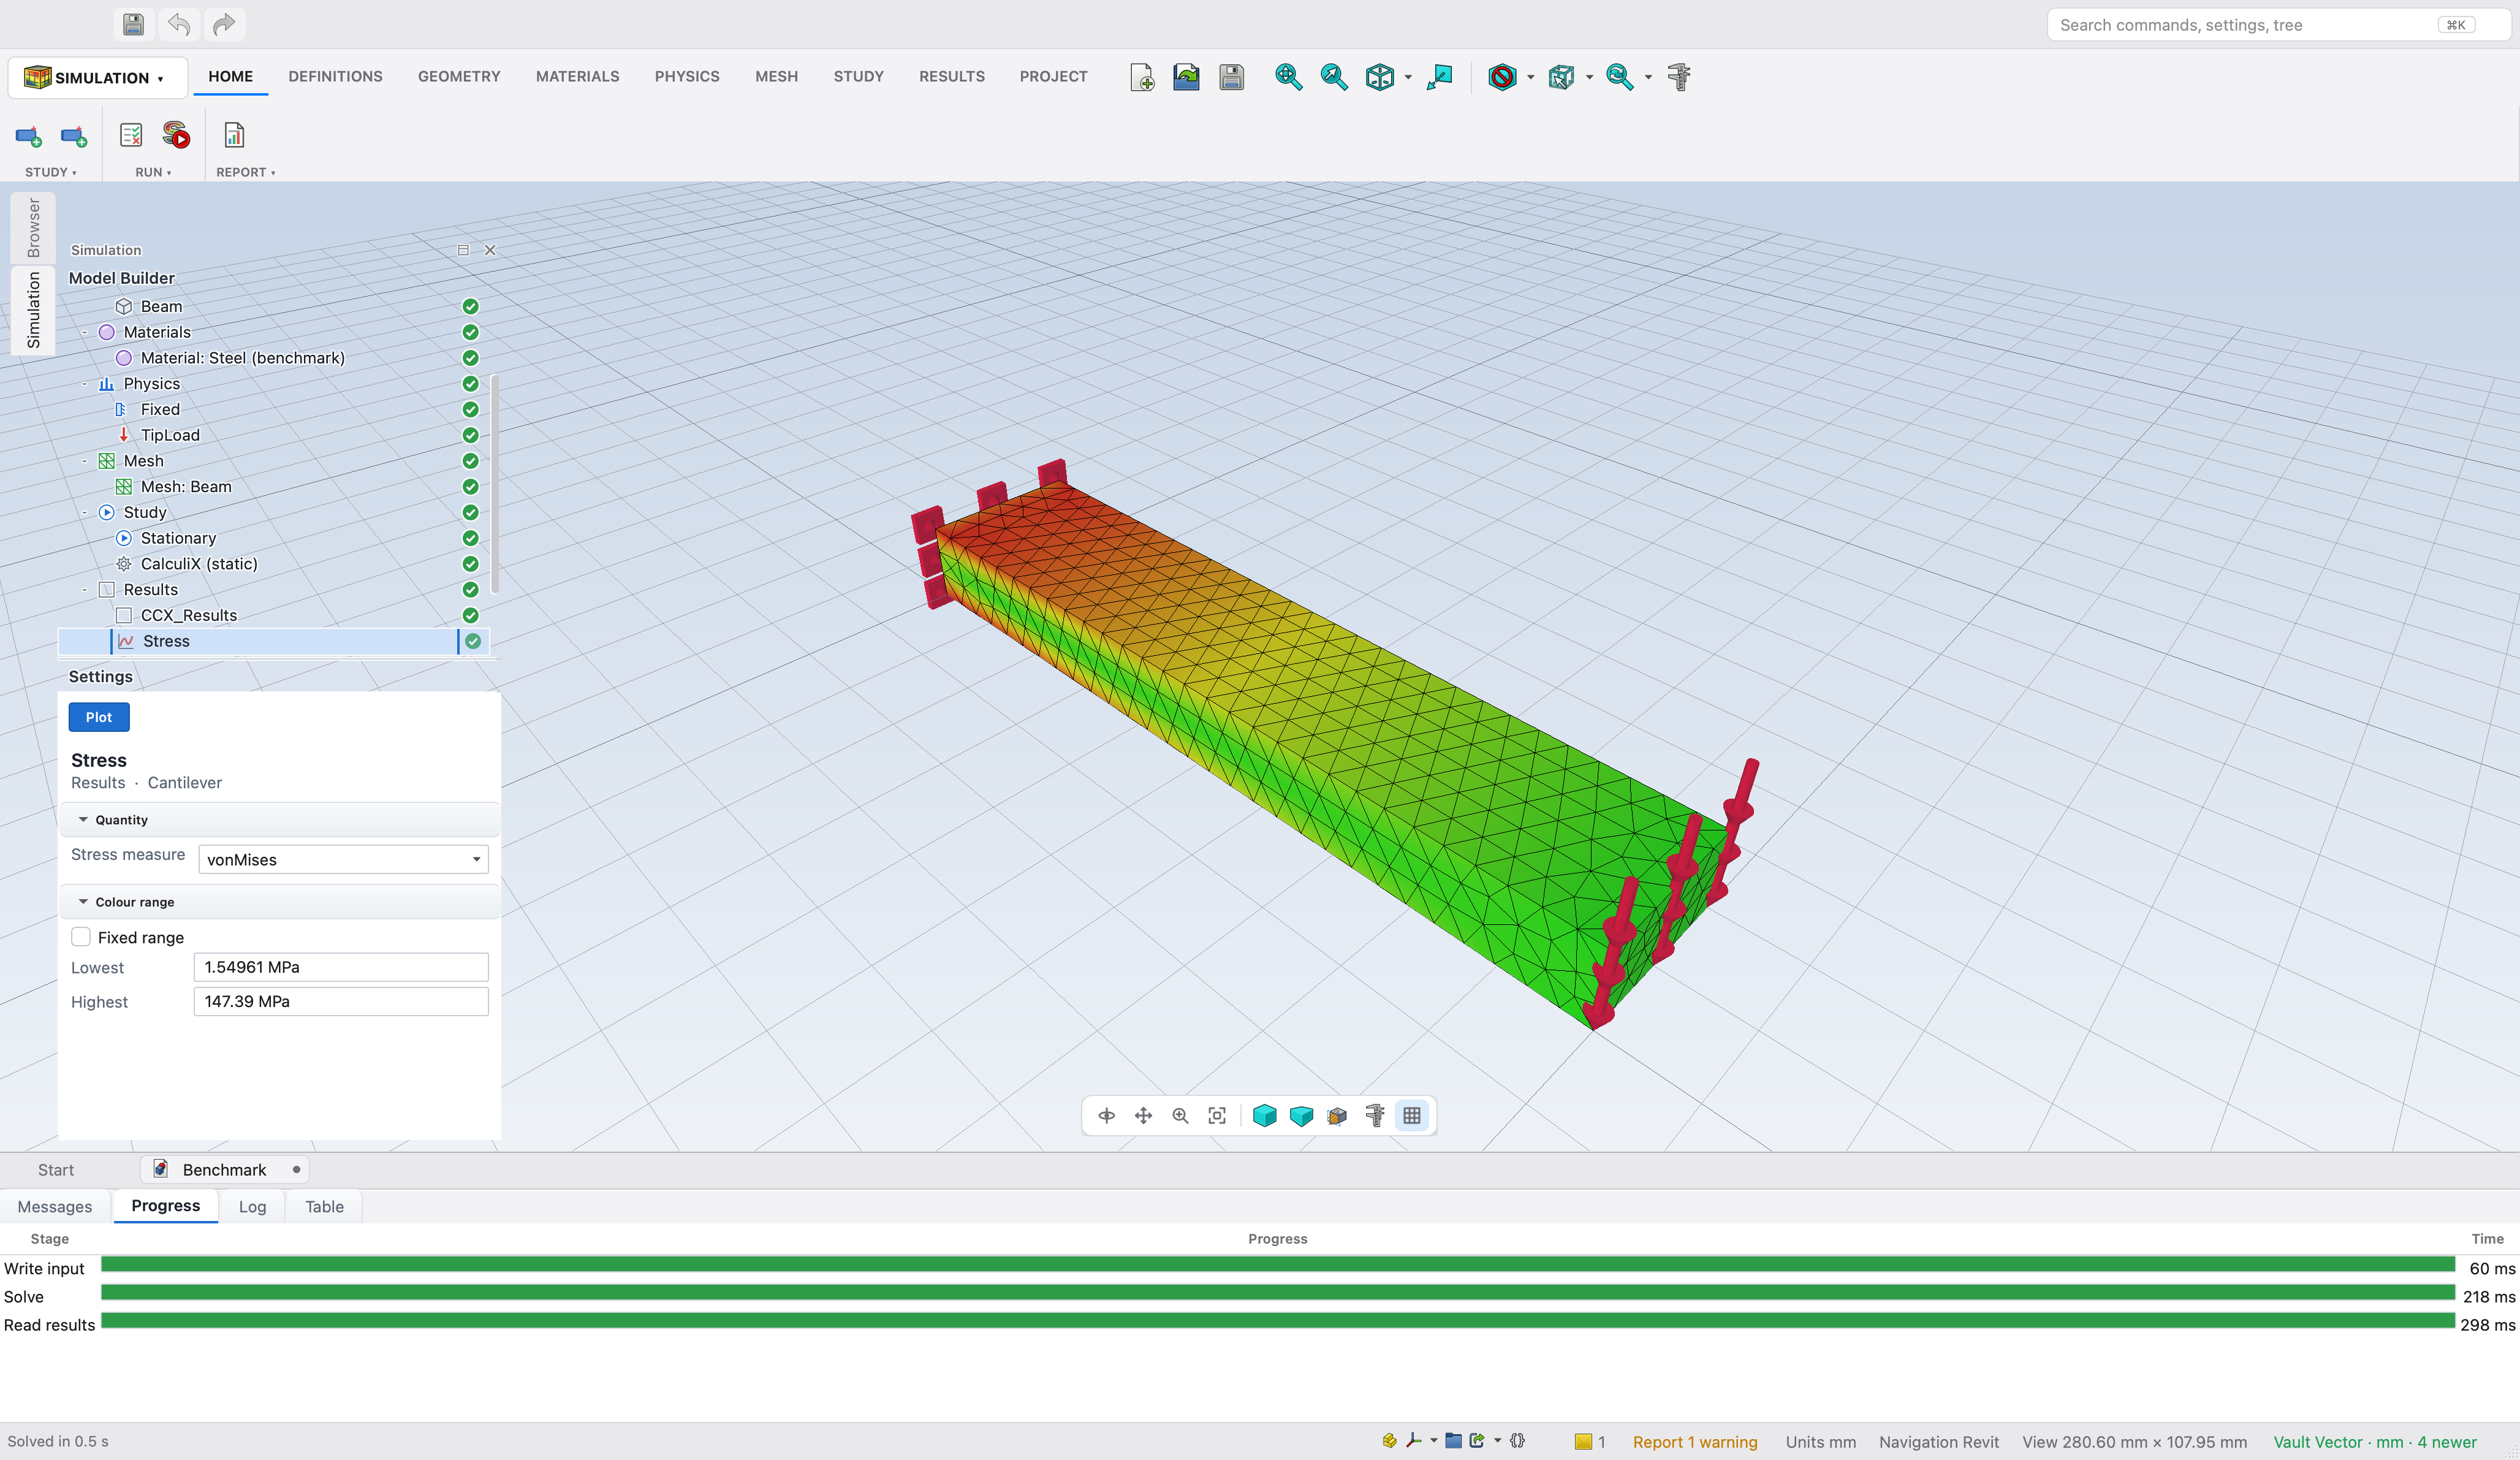
\includegraphics[width=\linewidth]{fig/simui_p1_results.png}
\caption{After \emph{Compute} from the Study node: the Progress tab shows the three stages, and the \emph{Stress} node under
Results is selected, which shows von Mises in the 3D view; its Settings hold the quantity and the fixed colour range.}
\label{fig:sim07-gui-results}
\end{figure}

\paragraph{What you can do now.}
\begin{itemize}[nosep]
  \item \textbf{The sidebar.} It is FreeCAD's own left overlay panel with a second tab, \emph{Simulation}; entering the
        workspace selects it, and the model tree is one click away on the \emph{Browser} tab. The panel is widened to
        400\,px for the tab and put back on leaving (see Horizontal tabs below). Inside the tab a splitter divides the Model Builder from Settings
        (Ansys' Outline and Details). The Messages, Progress, Log and Table dock stays under the graphics; the right panel
        stays put away. The earlier \emph{Model tree} header button, the auto hide of the tree and the 1500\,px switch
        are gone.
  \item \textbf{Model Builder.} A tree of \code{model\_tree(analysis)} with 21\,px rows, a node icon at the left and the
        state mark at the right (up to date, out of date, warning, needs attention, running, not set up); the icons are
        26 SVG files, one per symbol of the mockup sprite (\file{Resources/icons/sim/}, installed through CMake). It refreshes
        150\,ms after the active study changed, a value was set, the document recomputed or an object was created, changed
        or deleted, and when a mesh or solve ends. The pre-check findings are cached: a plain refresh reuses them, an
        airflow study recomputes them only after Compute (its pre-check tessellates the model). A tooltip names the reason
        for a mark. Selecting a message in the Messages pane that carries a node key selects that node.
  \item \textbf{Right-click.} Under Physics: \emph{Add} Fixed, Displacement, Force, Pressure, Spin (static) or Temperature,
        Heat flux, Convection, Heat source (thermal); the new node is selected, ready for faces. Mesh and Study: Compute,
        Pre-check. Result nodes: Plot. Loads, supports and results: Rename and Delete (one undo step each).
  \item \textbf{Settings.} A form from \code{settings(node)}: folding sections, a 96\,px label column, 22\,px fields,
        the unit written in the field (\code{500 N}), a number or an expression with a unit typed back (\code{2 kN},
        \code{12000 rpm}, \code{20 degC}); a wrong unit or a value out of range shows the model's text in red under the
        field and writes nothing; a good value goes through \code{set\_value} (one undo step) and the field shows the
        normalised value. Enums are combo boxes, switches check boxes, vectors three fields.
  \item \textbf{Faces.} While a node with a Selection field is current, a click on a face, edge or vertex of the part
        \emph{toggles} it (a plain click, no modifier: a click adds it, a click on a listed one removes it); the node's
        elements stay selected in the 3D view; the panel never closes. The part is shown (the mesh and result meshes put
        away) so its faces can be clicked. A Direction or axis field has a \emph{Pick in 3D view} button: the next click
        sets it.
  \item \textbf{Compute.} The Mesh node's button meshes. The Study node's (also on the step, solver and Results nodes)
        runs the pre-check (findings to Messages), meshes if needed, writes the input, solves in the Study panel's
        QProcess (the window stays live) and reads the results, with the events going to Progress, Log and Messages; the node
        shows the running mark meanwhile. On the blocking path the solver's own lines now reach the Log too. Airflow studies
        still run through the airflow panel (it opens).
  \item \textbf{Results.} Selecting a result node shows its field: Stress, Displacement, Safety factor, Hoop, Temperature
        (HDT bands when set), a mode shape, a solver result object, or the airflow results. Stress, Displacement and Hoop have
        a \emph{Colour range} section (Fixed range, lowest, highest), stored per study and field as before.
  \item \textbf{Ribbon.} The Study and Results tabs are hidden while no study is active; they come back with one.
\end{itemize}

\paragraph{Decided while building.}
\begin{itemize}[nosep]
  \item \textbf{Horizontal tabs (your choice, 1 Nov).} A strip across the top of the left panel, \emph{Browser $|$ Simulation},
        with the look of the right panel's (same \code{bwRightTabs} / \code{bwRightTab} styles and the same \code{bwTabStrip}
        panel switch, which takes the native tab bar out and shows one dock at a time); only the small strip class is
        new, since the right panel's own is bound to its docks and badges. Entering Simulation selects the Simulation
        tab. Outside the workspace there is no strip and only the Browser shows (hidden tab, switch off, the docks' own title
        rows back). The fork's \code{DockOverlayHideTabBar} setting is never touched, so nothing can be left set in a profile.
  \item \textbf{The Simulation tab stays registered.} An overlay panel cannot give a dock back, so leaving hides the tab (and
        the tab bar) and selects the Browser; the dock itself stays in the panel.
  \item \textbf{Widening the panel} uses the size grip's \code{dragMove} signal (invokable from Python; the panel's own slot is
        protected). No C++ was touched.
  \item \textbf{One click toggles.} No shift modifier: in a list that is being edited a click on a face is either an add or a
        remove, which the list tells at once.
  \item \textbf{Compute reuses the Study panel} as its run engine (never shown as a task panel), so the QProcess path, the
        events and the result display stay one code path until the old panels are retired.
  \item \textbf{The axis triad.} \code{hasAxisCross()} is true in the workspace. The triad (like the navigation cube) is a
        feedback visual of the live 3D widget and \code{saveImage} never draws it (checked: the same image with the triad on
        and off differs only in noise), so it is missing from off-screen renders and not from the window.
\end{itemize}

\paragraph{Tests.} \file{TestBruceWorxSimWorkspace} (28, 8 of them new for the panes): trees for static, modal, thermal and
prop-wash studies with 21\,px rows; marks after Compute, then after editing a Force (solution and results stale, mesh not),
a wrong unit and a negative force shown inline with the value and the undo stack unchanged, \code{2 kN} normalised;
face add and remove through the selection handler with the 3D highlight; mesh and solve from the pane buttons on the
cantilever, result nodes showing their field and the fixed range; the solver output in the Log on the blocking path;
adding, renaming, deleting (and undoing) a load and a message click selecting its node; refreshes debounced to one; the
sidebar tab, its splitter, the Browser tab, the tab bar and the fork's setting restored on leaving; the ribbon without Study
and Results tabs for no study. \file{TestBruceWorxSimulation}, \file{TestBruceWorxSimModel}, \file{TestBruceWorxWorkspaces}
and \file{TestBruceWorx} pass.

\paragraph{Open questions for you.}
\begin{enumerate}[nosep]
  \item \textbf{Highlight in renders.} The selection highlight and the triad do not appear in off-screen renders; they were
        checked through the selection state only. Please look at them in the real window.
  \item \textbf{Airflow Compute} still opens the airflow panel; its own node settings and pre-check cache are in the panes.
\end{enumerate}
